
\documentclass[main_ppt.tex]{subfiles}
%\usetikzlibrary{arrows}
%\usepackage{verbatim}

\tikzset{
  load/.style   = {ultra thick,-latex},
  stress/.style = {-latex},
  dim/.style    = {latex-latex},
  axis/.style   = {-latex,black!55},
}

\begin{document}

%\tikzset{
%  load/.style   = {ultra thick,-latex},
%  stress/.style = {-latex},
%  dim/.style    = {latex-latex},
%  axis/.style   = {-latex,black!55},
%}

% Drawing View
\tikzset{dimetric2/.style={
  x={(0cm,1cm)},
  y={(1cm,0cm)},
  z={(0cm,0cm)},
}}


%\begin{tikzpicture}
%      \coordinate (O) at (5,10,0); 
%       \draw[axis] (O) -- ++(0.5,0,0) %node[below right] {$x$};
%       \draw[axis] (O) -- ++(0,0.5,0) %node[above left] {$y$};
      % \draw[axis] (O) -- ++(0,0,0.5) node[above] {$z$};


%\draw[thick] (0,0,0) -- (10,0,0);
%\draw[thick] (0,0,0) -- (0,5,0);
%\draw[thick] (10,5,0) -- (0,5,0);
%\draw[thick] (10,5,0) -- (10,0,0);
%\end{tikzpicture}

\begin{tikzpicture}

     % \coordinate (O) at (0,-0.25,0); 
     %  \draw[axis] (O) -- ++(0.5,0,0) node[below right] {$x$};
     %  \draw[axis] (O) -- ++(0,0.5,0) node[above left] {$y$};




 \node[anchor=south west, inner sep = 0](image) at (0,0,0) {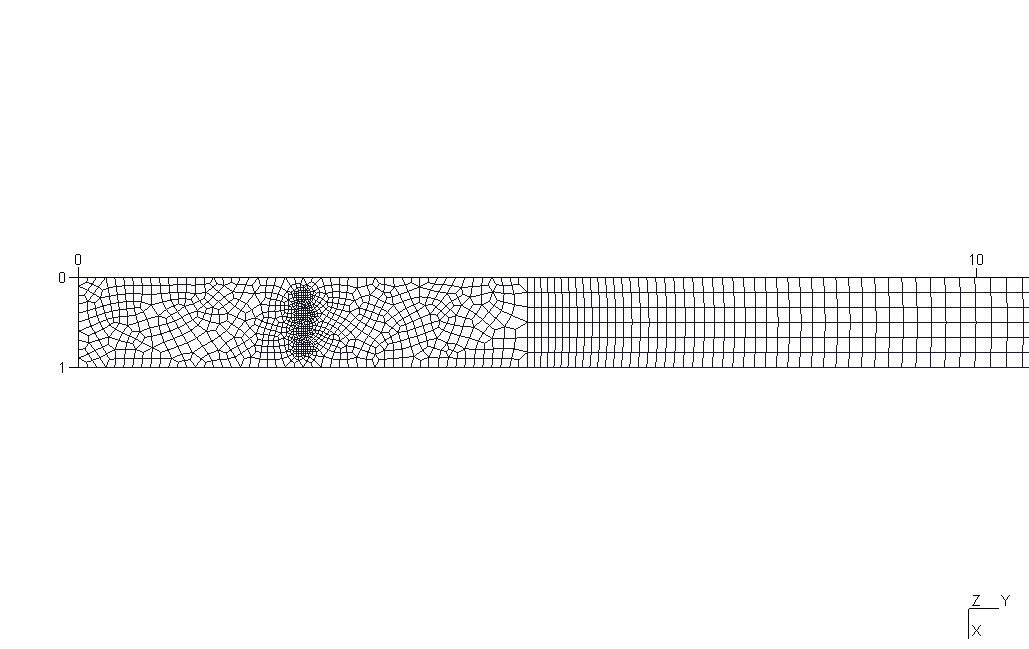
\includegraphics[width=\linewidth,trim={0cm 8cm 0cm 8cm},clip]{ParaStudy_onlydata/Mesh_Dependency/meshes/strip.png}};
 
%\draw[red] (5.55,1.05) -- +(1.1in,-0.6in)node[anchor=west] {Sampling Point};
 
%\draw[red] (5.55,1.505) -- +(1.1in,-0.6in)node[anchor=west] {Sampling Point};

%\draw[red] (5.55,0.6) -- +(1.1in,-0.6in)node[anchor=west] {Pn3};

%\draw[green] (0.85,1.505) -- +(0in,-0.38in)node[anchor=north] {$U(t)=sin(wt)$} ;
  
\draw (0.83,1.9) -- (0.83,2.3) ;
\draw (5.55,1.605) -- (5.55,2.3) ;
\draw[dim] (0.83,2.1) -- (5.55,2.1) node [midway,below] {$5m$} ;



\draw[blue,variable=\x,samples at={0,0.02,...,2}] plot({\x+2},{0.5*sin(4*\x r)-0.8},0);

%\draw[green,->] (0.5,-0.5,0) -- (3.5,-0.5,0) node [right] {$t$};
\draw[->] (2,-0.8,0) -- (4,-0.8,0) node [right] {$t$};
\draw[->] (2,-0.8,0) -- (2,0,0) node [right] {$w$};

\draw[blue,->] (1.9,-0.8,0) -- (0.85,1.05,0) ;

%\draw[->] (0.5,-0.5,0) -- (3.5,-0.5,0) node [right] {$t$};
%\draw[->] (0.5,-0.5,0) -- (0.5,0.5,0) node [right] {$t$};
%draw[green] (0.85,1.505) -- +(0in,-0.38in)node[anchor=north] {$U(t)=sin(wt)$} ;



\draw[red,variable=\x,samples at={0,0.02,...,2}] plot({\x+5},{0.5*sin(4*\x r)-0.8},0);

%\draw[green,->] (0.5,-0.5,0) -- (3.5,-0.5,0) node [right] {$t$};
\draw[->] (5,-0.8,0) -- (7,-0.8,0) node [right] {$t$};
\draw[->] (5,-0.8,0) -- (5,0,0) node [right] {$F$};

\draw[red,->] (4.9,-0.8,0) -- (3.2,1.05,0) ;



\end{tikzpicture}


\end{document}

